%%%%%%%%%%%%%%%%%%%%%%%%%%%%%%%%%%%%%%%%%
% University Assignment Title Page 
% LaTeX Template
% Version 2.1 (18/10/18)
% Modified by
% Erdem TUNA &
% Halil TEMURTAŞ &
% Enes TAŞTAN
%%%%%%%%%%%%%%%%%%%%%%%%%%%%%%%%%%%%%%%%%
%
%----------------------------------------------------------------------------------------
%	PACKAGES AND OTHER DOCUMENT CONFIGURATIONS
%----------------------------------------------------------------------------------------
\documentclass[a4paper,12pt]{article}
%-----packages------
\usepackage[a4paper, total={6.2in, 9in}]{geometry}
\usepackage[english]{babel}
\usepackage[utf8x]{inputenc}
\usepackage{amsmath}
\usepackage{graphicx}
\usepackage[colorinlistoftodos]{todonotes}
\usepackage{gensymb} % this could be problem
\usepackage{float}
\usepackage{fancyref}
\usepackage{subcaption}
\usepackage[titletoc]{appendix} %appendix package
\usepackage{xcolor}
\usepackage{listings}
\usepackage{xspace}
\usepackage{amssymb}
\usepackage{nicefrac}
\usepackage{gensymb}
\usepackage{fancyhdr}
\usepackage{lipsum}  % for dummy text \lipsum[1-4]
\usepackage[final]{pdfpages}  % pdf include
%\usepackage{array} %allows more options in tables
\usepackage{pgfplots,pgf,tikz} %coding plots in latex
%\usepackage{capt-of} % allows caption outside the figure environment
\usepackage[export]{adjustbox} %more options for adjusting the images
%\usepackage{multicol,multirow,slashbox} % allows tables like table1
%\usepackage[hyperfootnotes=false]{hyperref} % clickable references
%\usepackage{epstopdf} % useful when matlab is involved
%\usepackage{placeins} % prevents the text after figure to go above figure with \FloatBarrier 
%\usepackage{listingsutf8,mcode} %import .m or any other code file mcode is for matlab highlighting

%-----end of packages

%-----specifications-----
\definecolor{mGreen}{rgb}{0,0.6,0} % for python
\definecolor{mGray}{rgb}{0.5,0.5,0.5}
\definecolor{mPurple}{rgb}{0.58,0,0.82}
\definecolor{mygreen}{RGB}{28,172,0} % color values Red, Green, Blue for matlab
\definecolor{mylilas}{RGB}{170,55,241}

\setcounter{secnumdepth}{5} % how many sectioning levels to assign numbers to
\setcounter{tocdepth}{5}    % how many sectioning levels to show in ToC

\lstdefinestyle{CStyle}{
	commentstyle=\color{mGreen},
	keywordstyle=\color{magenta},
	numberstyle=\tiny\color{mGray},
	stringstyle=\color{mPurple},
	basicstyle=\footnotesize,
	breakatwhitespace=false,         
	breaklines=true,
	frame=single,
	rulecolor=\color{black!40},                 
	captionpos=b,                    
	keepspaces=true,                 
	numbers=left,                    
	numbersep=5pt,                  
	showspaces=false,                
	showstringspaces=false,
	showtabs=false,                  
	tabsize=2,
	language=C
}

\lstset{language=Matlab,%
	%basicstyle=\color{red},
	breaklines=true,%
	frame=single,
	rulecolor=\color{black!40},
	morekeywords={matlab2tikz},
	keywordstyle=\color{blue},%
	morekeywords=[2]{1}, keywordstyle=[2]{\color{black}},
	identifierstyle=\color{black},%
	stringstyle=\color{mylilas},
	commentstyle=\color{mygreen},%
	showstringspaces=false,%without this there will be a symbol in the places where there is a space
	numbers=left,%
	numberstyle={\tiny \color{black}},% size of the numbers
	numbersep=9pt, % this defines how far the numbers are from the text
	emph=[1]{for,end,break},emphstyle=[1]\color{red}, %some words to emphasise
	%emph=[2]{word1,word2}, emphstyle=[2]{style},    
}


\tikzset{
	desicion/.style={
		diamond,
		draw,
		text width=4em,
		text badly centered,
		inner sep=0pt
	},
	block/.style={
		rectangle,
		draw,
		text width=10em,
		text centered,
		rounded corners
	},
	cloud/.style={
		draw,
		ellipse,
		minimum height=2em
	},
	descr/.style={
		fill=white,
		inner sep=2.5pt
	},
	connector/.style={
		-latex,
		font=\scriptsize
	},
	rectangle connector/.style={
		connector,
		to path={(\tikztostart) -- ++(#1,0pt) \tikztonodes |- (\tikztotarget) },
		pos=0.5
	},
	rectangle connector/.default=-2cm,
	straight connector/.style={
		connector,
		to path=--(\tikztotarget) \tikztonodes
	}
}

\tikzset{
	desicion/.style={
		diamond,
		draw,
		text width=4em,
		text badly centered,
		inner sep=0pt
	},
	block/.style={
		rectangle,
		draw,
		text width=10em,
		text centered,
		rounded corners
	},
	cloud/.style={
		draw,
		ellipse,
		minimum height=2em
	},
	descr/.style={
		fill=white,
		inner sep=2.5pt
	},
	connector/.style={
		-latex,
		font=\scriptsize
	},
	rectangle connector/.style={
		connector,
		to path={(\tikztostart) -- ++(#1,0pt) \tikztonodes |- (\tikztotarget) },
		pos=0.5
	},
	rectangle connector/.default=-2cm,
	straight connector/.style={
		connector,
		to path=--(\tikztotarget) \tikztonodes
	}
}
%-----end of specifications-----


%----commands----
\newcommand\nd{\textsuperscript{nd}\xspace}
\newcommand\rd{\textsuperscript{rd}\xspace}
\newcommand\nth{\textsuperscript{th}\xspace} %\th is taken already
\newcommand{\specialcell}[2][c]{ \begin{tabular}[#1]{@{}c@{}}#2\end{tabular}} % for too long table lines

\newcommand{\blankpage}{
	\- \\[9cm]	
	{ \centering \textit{This page intentionally left blank.} \par }
	\- \\[9cm]
}% For Blank Page

\makeatletter
\renewcommand\paragraph{\@startsection{paragraph}{4}{\z@}%
	{-2.5ex\@plus -1ex \@minus -.25ex}%
	{1.25ex \@plus .25ex}%
	{\normalfont\normalsize\bfseries}}
\makeatother
%-----end of commands-----

\begin{document}

\begin{titlepage}

\newcommand{\HRule}{\rule{\linewidth}{0.5mm}} % Defines a new command for the horizontal lines, change thickness here
\centering 


\includegraphics[width=\textwidth,height=\textheight,keepaspectratio]{../../Documents/logos/logo3-with-stroke}\\[0.5cm]

\textsc{\LARGE Middle East Technical University}\\[0.5cm] % Name of your university/college
\textsc{\Large Department of \\Electrical and Electronics Engineering }\\[0.5cm] % Major heading such as course name
\textsc{\large EE493 ENGINEERING DESIGN I}\\[0.5cm] % Minor heading such as course title


\HRule \\[0cm]
{ \huge \bfseries  Car Chasing Robot\\[0.1cm] \LARGE \bfseries Proposal Report}\\[0cm] % Title of your document
\HRule \\[1cm]

\begin{minipage}[l]{0.6\textwidth}
\raggedright
		\large{\textbf{Supervisor:}}	Assoc. Prof. Emre Özkan \\
		\hspace{3.05cm}\color{red} ADDDRESSS

\end{minipage}
\begin{minipage}[r]{0.35\textwidth}
\raggedright
		\textbf{Project Start:} 4/10/2018\\
		\textbf{Project End:} \ \  26/5/2019\\
		\textbf{Project Budget:} \$450

\end{minipage}\\[1cm]
\begin{minipage}{\textwidth}
	\begin{flushleft}
		\large{\textbf{Company Name :}}	Duayenler Ltd. Şti.\\
		\begin{table}[H]
			\begin{tabular}{l l l l}
				\hline
				\textbf{Members}&\textbf{Title}& \textbf{ID}&\textbf{Phone} \\ \hline
				Sarper Sertel & Electronics Engineer& 2094449 & 0542 515 6039  \\ 
				Enes Taştan & Hardware Design Engineer & 2068989 & 0543 683 4336  \\ 
				Erdem Tuna & Embedded Systems Engineer& 2617419 & 0535 256 3320  \\ 
				Halil Temurtaş & Control Engineer& 2094522 & 0531 632 2194  \\
				İlker Sağlık & Software Engineer& 2094423 & 0541 722 9573  \\ \hline
				
				
			\end{tabular}
		\end{table}
	\end{flushleft}
\end{minipage}\\[1cm]

\begin{flushbottom}
{\large November 9, 2018} % Date, change the \today to a set date if you want to be precise
\end{flushbottom}

\end{titlepage}

%\blankpage
\tableofcontents
\newpage


	\section{notes}
\subsection{problem statement, societal impact of the project,}

\subsection{company organization (human resources, etc.),}


\subsection{specific requirements and objectives of the project}


\subsection{approach to the solution of the problem}


\subsection{outline of the requirements for any standards that the product would need to comply with,}


\subsection{deliverables and expected outcomes of the project,}


\subsection{tentative cost-budget analysis,}

\subsection{time plan (Gantt chart),}



\section{Executive Summary}


\section{Introduction}


\section{Team Organization}


\section{Requirement Analysis}

\begin{figure}[H]
	\centering
	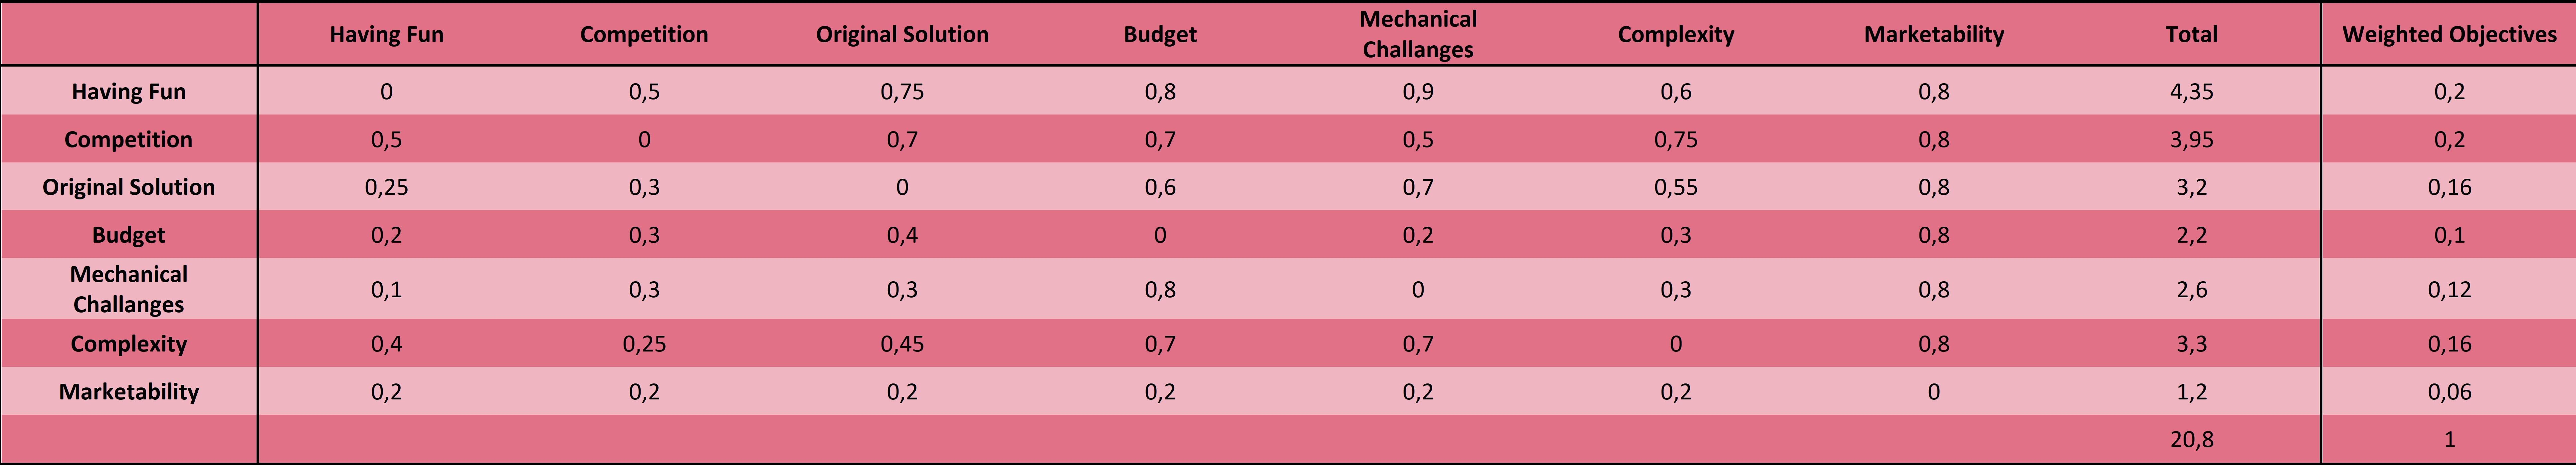
\includegraphics[width=\textwidth,height=\textheight,keepaspectratio]{images/objective_tree} 
	\caption{\label{fig:schedule}Weekly Schedule}
	
\end{figure}

\begin{figure}[H]
	\centering
	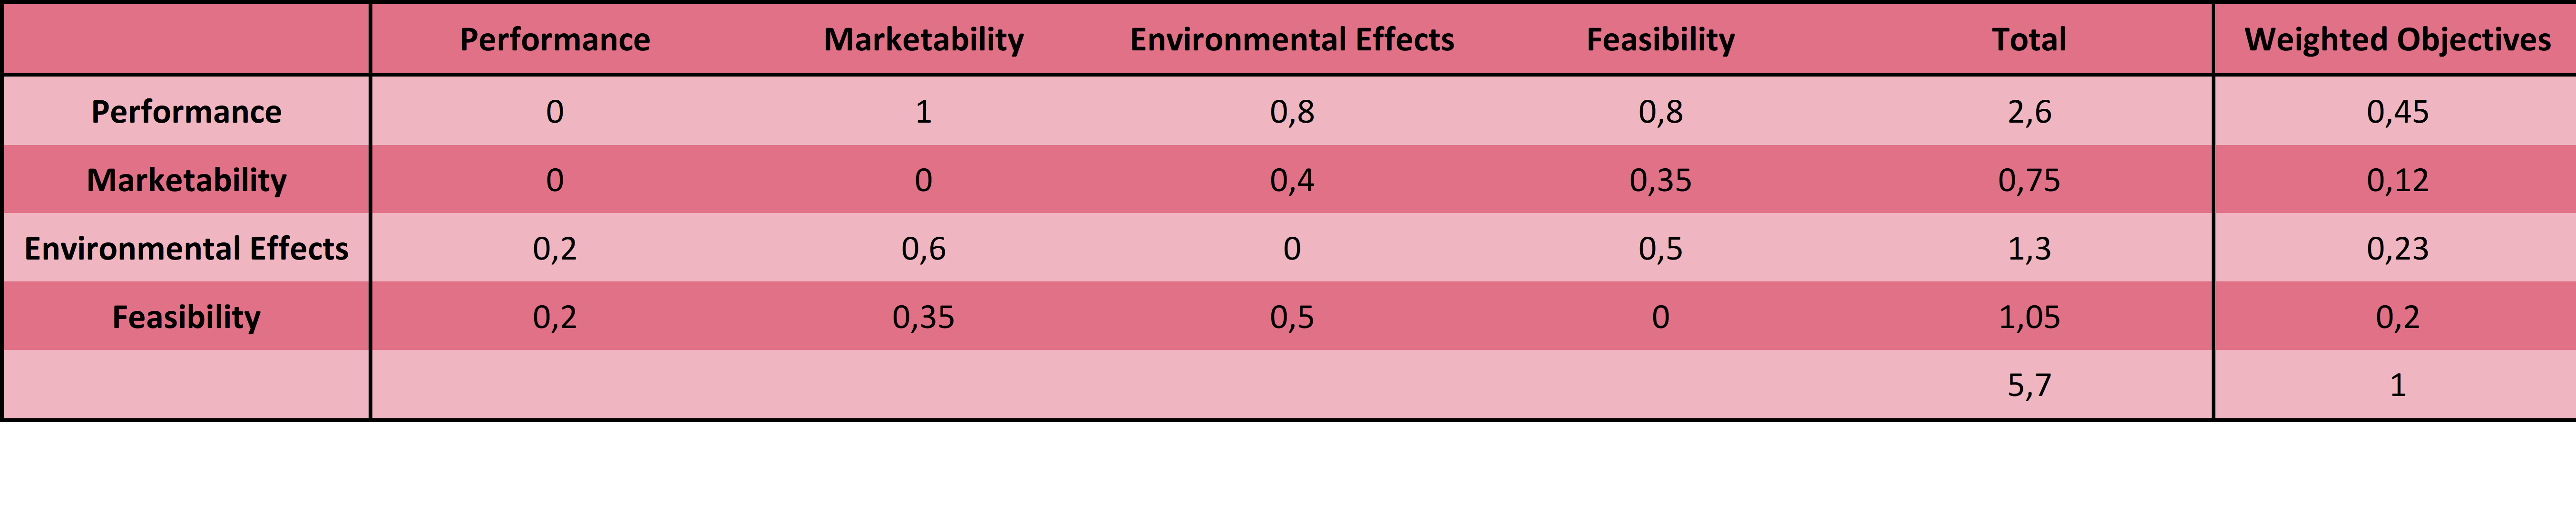
\includegraphics[width=\textwidth,height=\textheight,keepaspectratio]{images/proje_objective_tree} 
	\caption{\label{fig:schedule}Weekly Schedule}
	
\end{figure}


\begin{figure}[H]
	\centering
	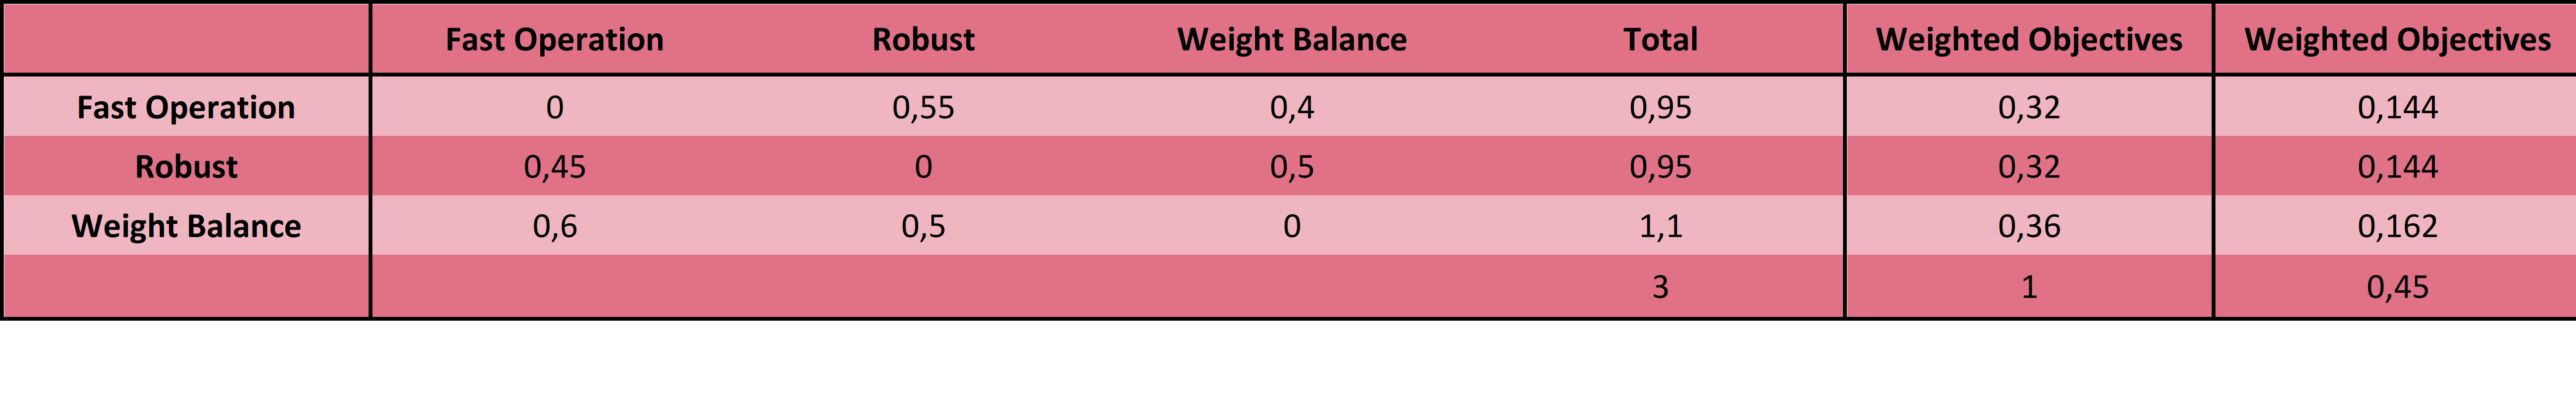
\includegraphics[width=\textwidth,height=\textheight,keepaspectratio]{images/proje_objective_tree_2} 
	\caption{\label{fig:schedule}Weekly Schedule}
	
\end{figure}


\begin{figure}[H]
	\centering
	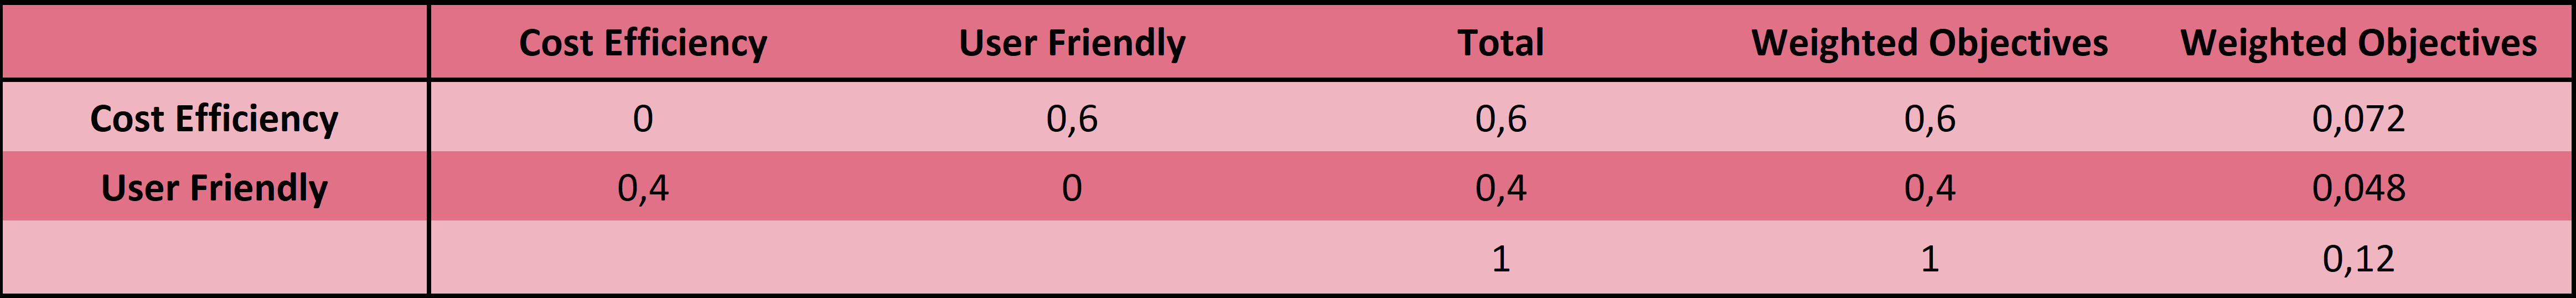
\includegraphics[width=\textwidth,height=\textheight,keepaspectratio]{images/proje_objective_tree_3} 
	\caption{\label{fig:schedule}Weekly Schedule}
	
\end{figure}


\begin{figure}[H]
	\centering
	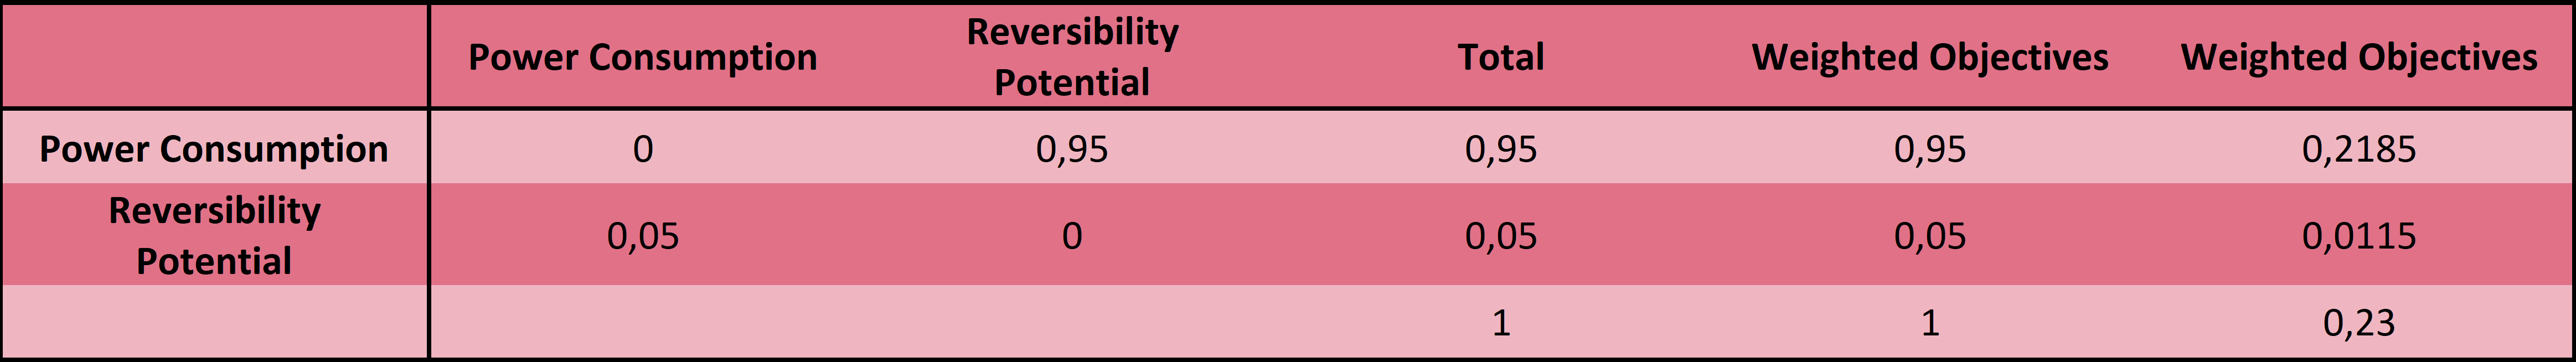
\includegraphics[width=\textwidth,height=\textheight,keepaspectratio]{images/proje_objective_tree_4} 
	\caption{\label{fig:schedule}Weekly Schedule}
	
\end{figure}

\begin{figure}[H]
	\centering
	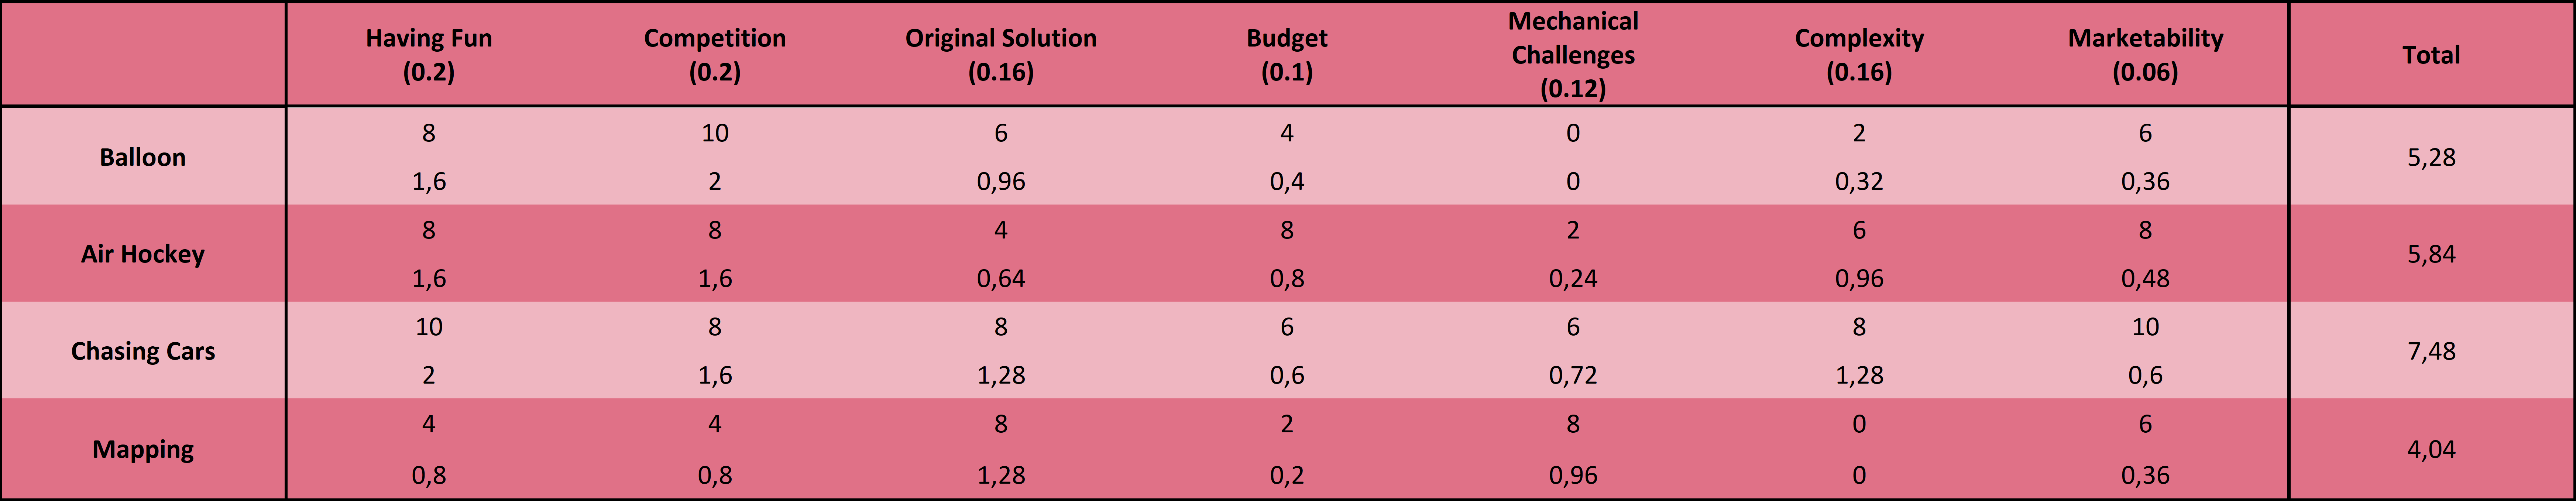
\includegraphics[width=\textwidth,height=\textheight,keepaspectratio]{images/project_evaluation} 
	\caption{\label{fig:schedule}Weekly Schedule}
	
\end{figure}


\section{Standards Section}


\section{Solution Procedure}


\section{Expected Deliverables}


\todo{Is the problem sufficiently important to justify money, company time, and your effort?}

\todo{Is the project well defined and realistic?}

\todo{Have you outlined a sound approach, including your ability to perform the tasks?}

\section{Conclusion}
	
\begin{appendices}
	
	


	
\end{appendices}




\end{document}

%----samples------
%\begin{itemize}
%\item Item
%\item Item
%\end{itemize}

%\begin{figure}[H]
%\center
%\setlength{\unitlength}{\textwidth} 
%
\includegraphics[width=0.7\unitlength]{images/logo1}
%\caption{\label{fig:logo}Logo }
%\end{figure}

%\begin{figure}[H]
%	\setlength{\unitlength}{\textwidth} 
%	\centering
%	\begin{subfigure}{.5\textwidth}
%  		\centering
%  		
\includegraphics[width=0.48\unitlength]{images/logo1}
%  		\caption{\label{fig:logo1}Logo1 }
%	\end{subfigure}%
%	\begin{subfigure}{.5\textwidth}
%  		\centering
%		
\includegraphics[width=0.48\unitlength]{images/logo2}
%  		\caption{\label{fig:logo2}Logo2}
%	\end{subfigure}
%\caption{\label{fig:calisandegree} Small Logos   }
%\end{figure}
	
%\begin{table}[H]
%  \centering
% 
%    \begin{tabular}{c|c|c}
%       $$A$$ & $$B$$ & $$C$$ \\ \hline
%       1 & 2 & 3  \\ \hline
%       2 & 3 & 4  \\ \hline
%       3 & 4 & 5  \\ \hline
%       4 & 5 & 6  
%      
%  \end{tabular}
%  \caption{table}
%  \label{tab:table}
%\end{table}
	
%\begin{table}[H]
%  \centering
% 
%    \begin{tabular}{c|c|c}
%       \backslashbox{$A$}{$a$} & $$\specialcell{ Average deviation \\ after subtracting out the  \\ frequency error }$$ & $$C$$ \\ \hline
%       \multirow{2}{*}{1} & 2 & 3  \\ \cline{2-3}
%        & 3 & 4  \\ \hline
%       3 & \multicolumn{2}{c}{4}  \\ \hline
%       4 & 5 & 6  
%      
%  \end{tabular}
%  \caption{table}
%  \label{tab:table}
%\end{table}
%-----end of samples-----